\chapter{Formalising ZKBoo}
\label{ch:formal_zkboo}

\begin{figure}[ht]
  \centering
  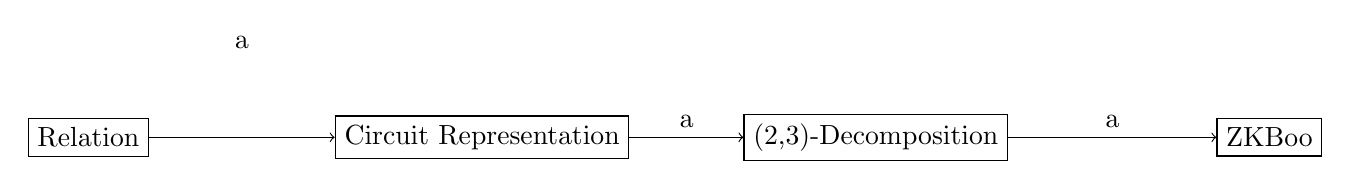
\begin{tikzpicture}
      \node[draw] at (-20,.3) (a) {Relation};
      \node[draw] at (-15,.3) (b) {Circuit Representation};
      \node[draw] at (-10,.3) (c) {(2,3)-Decomposition};
      \node[draw] at (-5,.3) (d) {ZKBoo};

      % draw edges
      \draw[->] (a) -- node[midway,above,yshift=1cm] {a} (b);
      \draw[->] (b) -- node[midway,above] {a} (c);
      \draw[->] (c) -- node[midway,above] {a} (d);
  \end{tikzpicture}
  \caption{\label{fig:outline_zkboo} Outline of ZKBoo formalisation}
\end{figure}

To formalise the ZKBoo protocol we need the following:

\begin{itemize}
  \item A formalisation of Arithmetic circuits
    \begin{itemize}
        \item With evaluation semantics
    \end{itemize}
  \item A formalisation of the (2,3)-Decomposition
    \begin{itemize}
      \item Proof of completeness
      \item Proof of 2-Privacy
    \end{itemize}
  \item An instantiation of a $\Sigma$-protocol for ``MPC in the head''
\end{itemize}

Thought out this section we assume that all challenges are sampled within the
set of $\{1,2,3\}$ and define that $3+1 = 1$.

\todo{Fran�ois et al. formalised Yao's protocol with a circuit representation
  similar to mine}

\section{Formalising Arithmetic circuits}
\label{sec:arith_circuits}
To express arbitrary computations in a ring of finite integer we need four
gates, namely, Add to constant (ADDC), multiply by constant (MULTC), addition of two wires (ADD),
and multiplication of two wires (MULT).

For an arithmetic circuit consisting of the aforementioned four gates we define the following notation:
\begin{definition}[Arithmetic Circuit]
  An Arithmetic circuit is a graph C = (W, G, i, o) where W is the internal wires between the gates and G is the set of gates within the circuit, finally i is the input gate and o is the designated output gate, for which there must exists a path from i to o in W.

  \dots
  \todo{parent/child nodes}
  \todo{Values flow through wires, but wires are not needed}
\end{definition}

To express in a well-defined way it is necessary to define a computational order. Since our circuit is expressed as a graph with a singular start and end node it is possible to define the notion of depth. The depth of a node n defined as the number of nodes between i and n.
Nodes at the same level can be computed in parallel since \dots

We simplify our notion of the computation order and remove all parallel computations. To achieve this we define a linear order on the gates by perform a breadth-first numbering of the nodes starting from the input gate i and ending at o.

By performing this we are ensure that no nodes are computed before their parent nodes have been computed.

\begin{lstlisting}[float,label=lst:gate_types,caption=Type declaration of gates]
type gate = [
  | ADDC of (int * int)
  | MULTC of (int * int)
  | MULT of (int * int)
  | ADD of (int * int)
].

type circuit = gate list.
\end{lstlisting}

This ordering allows us to convert the graph representation into a list
representation, where the gate at index $i$ is the node with index $i$ in the
BFS numbering of the graph.
But we need to encode W into this list. To do this we encode the information
about input wires into the types of the gates themselves, as seen in figure
\ref{lst:gate_types}. A gate is then a type, which defined its operation along
with a tuple $(l,r)$ where $l$ is the index of left input wire and $r$ is the
index of the right input wire. In the case of unary gates like ADDC and MULTC
the tuple is $(l, c)$ where l is the input wire and $c$ is the constant used in
the computation.

\begin{definition}[List representation of arithmetic circuits]
  To represent an arithmetic circuit as a list we \dots
\end{definition}

\todo{Tikz example showing the two representations}

\begin{definition}[Valid circuit]
  \label{def:decomp:valid_circuit}
  An arithmetic circuit in list representation C is valid if:
  \begin{itemize}
    \item For every entry $i$ in the list it holds that
      \begin{itemize}
        \item C[i] is a gate type
        \item the input wires of C[i] have index less than $i$.
        \item the input wires of C[i] have index greater than or equals to $0$.
      \end{itemize}
  \end{itemize}
\end{definition}

\begin{lstlisting}[float,label=lst:circuit_eval,caption=Circuit evaluation function]
op eval_gate (g : gate, s : int list) : int =
  with g = MULT inputs => let (i, j) = inputs in
                          let x = (nth 0 s i) in
                          let y = (nth 0 s j) in x * y
  with g = ADD inputs =>  let (i, j) = inputs in
                          let x = (nth 0 s i) in
                          let y = (nth 0 s j) in x + y
  with g = ADDC inputs => let (i, c) = inputs in
                          let x = (nth 0 s i) in x + c
  with g = MULTC inputs => let (i, c) = inputs in
                          let x = (nth 0 s i) in x * c.

op eval_circuit_aux(c : circuit, s : int list) : int list =
    with c = [] => s
    with c = g :: gs =>
     let r = eval_gate g s in
     eval_circuit_aux gs (rcons s r).

op eval_circuit (c : circuit, s : state) : output =
    last 0 (eval_circuit_aux c s).
\end{lstlisting}

By representing gates as types encoding wire information we can use \easycrypt's
type system to pattern matching system to perform computations relevant to the
gate type, as seen in \ref{lst:circuit_eval}.

From this representation of circuits as a list of gates, where gates are types,
it is possible to define the semantic meaning of this representation, by
defining the evaluation function, which can be seen in figure \ref{lst:circuit_eval}.
The evaluation is broken into two parts: one for evaluation one gate, and one
for evaluating the entire circuits, based on the former.
To evaluate one gate, we first need to determine which gate it is. This is done
by matching on the type of the gate.
Then, by the circuit being valid and the execution order follows the ordering of
indexes, we know that if we are computing index $i$ of the circuit, then indices
$[0 \dots i-1]$ have already been computed to an value representing the result
of computing the gate. Perform the appropriate function then simply reduces to
looking the values of the incoming wires and computing the function.

Computing the entire circuit then follows from the same fact, that gates are always
evaluated in the order the appear in the list, and the no gate can depend on
the result of gates, which have a higher index than itself. By continually
performing gate evaluation of the next entry in the list and saving the result
into ``state'' where each index correspond to the computed value of the gate at
that index in the circuit, and the calling recursively on the list with the
first entry removed, then the output of the gate will be in the last entry of
the state, when there are no more gates to compute. Assuming that there is only
one output gate.

``state'' can then be defined as
\begin{align*}
  \text{state}_{0} &= \text{input value} \\
  \text{state}_{i>0} &= \dots
\end{align*}

We then have that any valid circuit c can be compute to a value y as
\texttt{eval\_circuit(c, [input]) = y}. This can also be stated as a probabilistic
procedure as $\Pr{\texttt{eval\_circuit(c, [input])} = y} = 1$.

To reason about functions and procedures about functions we have the following lemma:
\begin{lemma}[Function/Procedure relation]
  \label{lem:func/proc-equiv}
  $\forall$ f, inputs, output: f(inputs) = output $\iff \Pr{f(inputs) = output} = 1$.
\end{lemma}


\section{(2,3) Decomposition of circuits}
\label{sec:decomposition}
In its most general form, we can define the decomposition as a procedure taking
as input three views and random tapes, and a circuit and produces three new
views.
More specifically the decomposition work by evaluating a gate based on
previously compute views, which yield new shares that can be appended to the
view. This process of evaluating a single gate based on the view of evaluating
the previous gate can then be repeated until all gates have been computed. This
overall idea has been captured in the procedure in figure \ref{lst:decomp_aux},
where it is assumed access to a function eval\_gate, which has signature:
$eval\_gate : circuit \Rightarrow party \Rightarrow (view * view) \Rightarrow (random\_tape * random\_tape) \Rightarrow share$,
where $party$ is a integer in $\{1,2,3\}$ that determines which party is
computing the share. \todo{Say that eval gate implements the function in the
  ZKBoo section}

\begin{lstlisting}[float,label=lst:decomp_aux,caption= Incremental decomposition procedure]
  proc compute(c : circuit, w1 w2 w3 : view, k1 k2 k3 : random_tape) = {
    while (c <> []) {
      g = oget (ohead c);
      r1 <$ dinput;
      r2 <$ dinput;
      r3 <$ dinput;
      k1 = (rcons k1 r1);
      k2 = (rcons k2 r2);
      k3 = (rcons k3 r3);
      v1 = eval_gate g 1 w1 w2 k1 k2;
      v2 = eval_gate g 2 w2 w3 k2 k3;
      v3 = eval_gate g 3 w3 w1 k3 k1;
      w1 = (rcons w1 v1);
      w2 = (rcons w2 v2);
      w3 = (rcons w3 v3);
      c = behead c;
    }
    return (k1, k2, k3, w1, w2, w3);
  }
\end{lstlisting}

The output of the decomposition can then be defined as summing the last share from each view that has been compute by the aformentioned procedure.

\todo{Define simulator...}

\todo{All functions and proof quantify over random tapes but they have been
  omitted from this write-up since they are just random values that need to be
  return to reconstruct the results}

\subsection{Randomness}
\label{subsec:decomp:randomness}
Throughout the decomposition we make a series of random choices to make the
shares random. These random choices are saved as a list, which we refer to as
the random tape. The reason of this is to be able to reconstruct the views given
the initial shares and the random choices. We chose to omit the details of the
random tapes. The reason for this is...


\subsection{Correctness}
\label{sec:decomp_correct}
Ultimately want to prove:
\begin{lemma}[Decomposition correctness]
  \label{lem:decomposition_correctness}

  \[
    \Pr{\texttt{eval\_circuit(c, [input])} = y} =
    \Pr{\texttt{decomposition(c, [input])} = y}
  \]

  i.e. The output distribution of the two programs are perfectly indistinguishable. From lemma \ref{lem:func/proc-equiv} we have that circuit evaluation always succeeds, this lemma, therefore, also implies that the decomposition always succeeds.
\end{lemma}

\begin{definition}[Correctness of views]
  \label{def:decomp:valid_view}
  For any three views (list of shares), $w_{1}, w_{2}, w_{3}$, with equal length, we
  say that they contain valid shares of computing a circuit c, if it holds:

  \[
          \forall 0 \leq i < size c,
              w_{1}[i] + w_{2}[i] + w_{3}[i] = s[i]
  \]

  where s is the list of intermediate values produces by calling
  \texttt{eval\_circuit\_aux} in figure \ref{lst:circuit_eval}.

  Additionally a share is only valid, if it has been produced by functions used
  by the decomposition.

  \[
    \forall e \in \{1, 2, 3\}
    \forall 0 \leq i < size c - 1,
      w_{e}[i + 1] = \texttt{phi\_decomp} c[i] 1 w_{e} w_{e+1} k_{e} k_{e+1} /\
  \]

  To express that the views satisfy the above definition we use the notation
  \validviews{c,w1,w2,w3} to express that $w1, w2, w3$ are valid views for the
  decomposition of $c$

\end{definition}

To prove the above lemma we first introduce a helper lemma:

\begin{lemma}[Stepping lemma for decomposition]
  \label{lem:decompose_compute_step}
  For any valid circuit c in list representation, it is possible to split the circuit into two parts
  $c_{1}, c_{2}$ where $c = c_{1} ++ c_{2}$ (++ is list concatenation).
  let $w_{1}, w_{2}, w_{3}$ be the resulting views of decomposing $c$ and
  \validviews{c_{1}, w_{1}, w_{2}, w_{3}} and let computing $c_{2}$ with initial
  views $w_{1}, w_{2}, w_{3}$ output views $w'_{1}, w'_{2}, w'_{3}$.
  Then \validviews{c, w'_{1}, w'_{2}, w'_{3}}.

  Alternatively this is stated as:
  \[
    \textbf{Valid}(c_{1}, w_{1}, w_{2}, w_{3})  \implies
    \Pr{ \texttt{compute}(c_{2}, w_{1}, w_{2}, w_{3}) : \textbf{Valid}(c, w'_{1} , w'_{2}, w'_{3}) } = 1
  \]

\end{lemma}
\begin{proof}
  The proof proceeded by induction on the list c.

  \begin{itemize}
    \item Base case $c = []$:
        trivially true since an empty circuit is the identity function.
    \item Induction step $c = c' ++ [g]$:
      \begin{itemize}
        \item Inline definitions to get compute\_stepped
        \item We use to induction hypotheses to compute c' which give us
              \validviews{c_{1}, w_{1}, w_{2}, w_{3}}.
        \item We then need to prove, that we can compute any gate on top of the
          valid views to produce a new set of valid views.
      \end{itemize}
  \end{itemize}

\end{proof}

\begin{proof}[Proof of lemma \ref{lem:decomposition_correctness}]
  By unfolding the definition we are left with proving that the last share from
  each of the views produced by \texttt{compute} are equal to the output of
  evaluating the circuit, which is true by lemma \ref{lem:decompose_compute_step}
\end{proof}

\todo{Our formalisation differs by imposing stricter restrictions on the shares computed...}


\subsection{2-Privacy}
\label{sec:decomp_privacy}
To prove 2-Privacy we need to first define a simulator capable of producing
indistinguishable views for two of the parties. To simulator is given by the
procedure \texttt{simulate} and function \texttt{simulator\_eval} in figure \ref{lst:zkboo:simulator}.
\texttt{simulator\_eval} is a function that evaluates a single gate from the
point of view of party ``p''. For the cases of evaluating ADDC ADD MULTC gates
the simulator simply calls the \texttt{eval\_gate} function, since these
computations are performed ``locally'' for each party, i.e. they do not depend
on the shares of the other two parties in the protocol.
When evaluating MULT gates shares needs to be distributed amongst the parties,
but to evaluate the output of the MULT gate for any given party it only depends
on the parties own share and the share of the ``next'' party, i.e. for party one
he only depends on the shares from himself and the shares from party two. Since
the simulator simulates the view of party $e$ and $e+1$ the view of party $e$
can be computed normally with the \texttt{eval\_gate} function. For simulating
the view of party $e+1$ we use the fact that shares should be uniformly random
distributed, and simply sample a random value for the view. In this case the
view of party $e$ can always be computationally reconstructed by looking at the
view of party $e+1$, but the view of party $e+1$ cannot be verified, since the
view of party $e+2$ is unknown, which makes it seem valid.

The procedure $\texttt{simulate}$ is simply a wrapper around
\texttt{simulator\_eval}, which is responsible for constructing the views and
sampling randomness.

\begin{lstlisting}[float,label=lst:zkboo:simulator,caption= Simulator]
op simulator_eval (g : gate, p : int, e : int, w1 w2 : view, k1 k2 k3: int list) =
with g = MULT inputs =>
  if (p - e %% 3 = 1) then (nth 0 k3 (size w1 - 1)) else eval\_gate g p w1 w2 k1 k2
with g = ADDC inputs =>
    eval\_gate g p w1 w2 k1 k2
with g = MULTC inputs => eval\_gate g p w1 w2 k1 k2
with g = ADD inputs => eval\_gate g p w1 w2 k1 k2.

proc simulate(c : circuit, e : int, w1 w2 : view, k1 k2 k3 : random_tape) = {
  while (c <> []) {
    g = oget (ohead c);
    r1 <$ dinput;
    r2 <$ dinput;
    r3 <$ dinput;
    k1 = (rcons k1 r1);
    k2 = (rcons k2 r2);
    k3 = (rcons k3 r3);
    v1 = simulator_eval g e e w1 w2 k1 k2 k3;
    v2 = simulator_eval g (e+1) e w2 w1 k1 k2 k3;
    w1 = (rcons w1 v1);
    w2 = (rcons w2 v2);
    c = behead c;
  }
\end{lstlisting}

To compare the views output by the simulator and the ones produced by the decomposition we fix two procedures \texttt{real} and \texttt{simulated}, where the first return two views and the final share of the third view and the latter returns the two views output by the simulator and a fake final share of the thrid view. These procedures can be seen in figure \ref{lst:decomp-real-ideal}.

\begin{lstlisting}[float, mathescape,label=lst:decomp-real-ideal,caption= Real/Simulated view of decomposition]

proc real((c,y) : statement, w : witness, e : challenge) = {
    $(y_{1},y_{2},y_{3},w_{1},w_{2},w_{3})$ = compute(c);
    return $(w_{e}, w_{e+1}, y_{e+2})$
}

proc simulated((c, y) : statement, e : challenge) = {
    $(w_{e}, w_{e+1})$ = simulate(c, e);
    $y_{e}$ = last $w_{e}$;
    $y_{e+1}$ = last $w_{e+1}$;
    $y_{e+2}$ = $y - (y_{e} + y_{e+1})$
    return $(w_{e}, w_{e+1}, y_{e+3})$
}

\end{lstlisting}

We are then ready to state 2-privacy as the following lemma:
\begin{lemma}[Decomposition 2-Privacy]
  \label{lem:zkboo:decomposition:privacy}
  We say that the decomposition protocol offers 2-Privacy, if the output
  distributions between \texttt{real} and \texttt{simulated} are
  indistinguishable.

  This can be stated in rPHL as:
  \[
    h \in \textbf{Domain}(R) \implies
    equiv[real \sim simulated : =\{e, h\} \implies =\{res\}].
  \]

\end{lemma}

To prove this lemma we first prove a that running \texttt{compute} and
\texttt{simulate} with the same random choices will produce indistinguishable
views corresponding to the challenge and summing the output shares of
\texttt{compute} will yield the same value as evaluating the circuit. This
effectively inlines the correctness property in the proof of the simulator. This
is necessary to be able to reason about the existence of the view of party
$e+2$, which would make the views produced by the simulated equal to honestly
produces views.
More specifically the inlined correctness property gives us ...

This is stated as the following lemma:

\begin{lemma}
  \label{lem:zkboo:decomposition:privacy_aux}
  Given a valid arithmetic circuit in list representation with challenge $e$ and
  intermediate circuit computations/state $s$ the following holds:

  \[
    equiv[compute \sim simulated : \; =\!\{h, e, w_{e}, w_{e+1}\} \implies =\!\{w'_{e}, w'_{e+1}\}]
  \]

  Moreover, we require that the input views to compute $w_{1}, w_{2}, w_{3}$ satisfy:
  \[
    \forall 0 \leq i < size w1, w_{1}[i] + w_{2}[i] + w_{3}[i] = s[i]
  \]

  Additionally this property most also hold for the views $w'_{1}, w'_{2}, w'_{3}$ produced by running \texttt{compute}. This is equivalent to part of the \textbf{Valid} property used in the proof of correctness.

  % \begin{itemize}
  %   \item Running \texttt{compute} and \texttt{simulate} with the same random
  %     choices satisfies conditions:
  %     \begin{itemize}
  %       \item The initial views of $w^{compute}_{e}$ and $w^{compute}_{e+1}$ are indistinguishable from  $w^{simulate}_{e}$ and $w^{simulate}_{e+1}$.
  %       \item It hold that $\forall 0 \leq i < size w1, w_{1}[i] + w_{2}[i] + w_{3}[i] = s[i]$
  %       \item
  %     \end{itemize}
  % \end{itemize}
\end{lemma}
\begin{proof}
  We proceed by induction on the list representation of the circuit c:

  \begin{itemize}
    \item Base Case $c = []$ : trivial
    \item Induction Case $c = g::cs$ :
    \item Write this as program steps like in \cite{certicrypt_sigma}?
      \begin{align*}
        compute(g::gs, w_{1}, w_{2}, w_{3}) \sim simulate(g::gs, w'_{1}, w'_{2}, w'_{3} )
      \end{align*}
  \end{itemize}

\end{proof}

\begin{proof}[Proof of lemma \ref{lem:zkboo:decomposition:privacy}]
  By applying lemma \ref{lem:zkboo:decomposition:privacy_aux} we have that the
  views output by both procedures are indistinguishable. All have left to prove
  is that $y^{real}_{e+2} \equiv y^{simulated}_{e+2}$. To prove this, we use the
  correctness definition, saying that the shares of the real views always sum to
  the intermediate values of computing the circuit, therefore:
  $y^{real}_{e+2} = y - (y^{real}_{e} + y^{real}_{e+1})$. Now, since
  $(y^{real}_{e} + y^{real}_{e+1}) \equiv (y^{real}_{e} + y^{real}_{e+1})$ it
  follows that
  \begin{align*}
    y^{simulated}_{e+2} &= y - (y^{simulated}_{e} + y^{simulated}_{e+1}) \\
                      &\equiv y - (y^{real}_{e} + y^{real}_{e+1}) \\
                      &= y^{real}_{e+2}
  \end{align*}
\end{proof}


\section{ZKBOO}
\label{sec:formal_zkboo}
Since the ZKBoo protocol is an instantiation of a $\Sigma$-Protocol we start by
defining the types as specified in section \ref{ch:formal_sigma} and
instantiating the $\Sigma$-Protocol framework.

\lstinputlisting[linerange={13-17}]{../code/ZKBoo.ec}

We then axiomatize that the challenge is always a integer in $\{1,2,3\}$. Since
it is not supported by the type system?

We assume the existence of an idealised commitment scheme which satisfies \dots

We then define a predicate for validating a view:
\lstinputlisting[linerange={47-54}]{../code/ZKBoo.ec}
Predicates allows us to use quantifiers to assert properties, which are nice to
reason about especially in pre and post condition of procedures. Predicates,
however, have no computation aspect to them and are pure logical. A predicate,
therefore, cannot be used within procedures, since they are not required to be
computable(?). We, therefore, add function which check the same properties, but
without the use of quantification. This requires us to use looping instead,
which can be harder to reason about.
Specially, it is much harder to reason about the $i$'th index of the view being
computed correctly given that valid\_view\_op returns true, whilst it immediately
follows from the predicate.

To bridge the gap between the computational and logical worlds we introduce the
following lemma:
\begin{lemma}[valid\_view predicate/op equivalence]
  $\forall$ p, w1, w2, c, k1, k2:
  valid\_view p w1 w2 c k1 k2 $\iff$ valid\_view\_op p w1 w2 c k1 k2
\end{lemma}

With a way to validate the views we can instantiate the ZKBoo protocol from
section \ref{sec:zkboo} as a $\Sigma$-Protocol in our formalisation by
implementing the algorithms from figure \ref{lst:sigma_procedures}, which can be
seen in figure \ref{lst:zkboo_procedures}.
\todo{Assumes existence of decomposition protocol}
\todo{Assumes existence of ideal commitment functionality}

\begin{lstlisting}[float, mathescape,label=lst:zkboo_procedures,caption= ZKBoo $\Sigma$-Protocol instantiation]
global variables = w1, w2, w3, k1, k2, k3.

proc init(h : statement, w : witness) = {
  (x1, x2, x3) = Share(w);
  (k1, k2, k3, w1, w2, w3) = Decompose(c, x1, x2, x3);
  $c_i$ = Commit($(w_{i}, k_i)$);
  $y_{i} = $ last 0 $w_{i}$;
  return (y1, y2, y3, w1, w2, w3);
}

proc response(h : statement, w : witness, m : message, e : challenge) = {
  return $(k_e, w_{e}, k_{e+1}, w_{e+1})$
}

proc verify(h : statement, m : message, e : challenge, z : response) = {
  (y1, y2, y3, c1, c2, c3) = m;
  (c, y) = h;

  (k1', w1', k2', w2') = open;
  valid_com1 = verify $(w'_{e}, k'_{e})$ c1;
  valid_com2 = verify $(w'_{e+1}, k'_{e+1})$ c2;
  valid_share1 = last 0 $w'_{e}$ = y1;
  valid_share2 = last 0 $w'_{e}$ = y2;
  valid = valid_view_op 1 $w'_{1}$ $w'_2$ c $k'_1$ $k'_2$;
  valid_length = size c = size $w'_e - 1$ /\ size $w'_{1}$ = size $w'_2$;

  return y = y1 + y2 + y3 /\ valid_com1 /\ valid_com2 /\ valid_share1 /\ valid_share2 /\ valid /\ valid_length
}

\end{lstlisting}

We then, automatically, by our formalisation of $\Sigma$-Protocols get definition of security and only need to prove them \dots \todo{wording}

\begin{lemma}
  \label{lem:zkboo:correctness}
  ZKBoo satisfy correctness definition \ref{def:sigma:completeness}.
\end{lemma}
\begin{proof}
We start by observing that committing to $(w_{i}, k_{i})$ in \texttt{init} and
the verifying the commitment in \texttt{verify} is equivalent to the correctness
game for commitment schemes defined in \ref{ch:formal_commitment}.

We therefore inline the completeness game, and replace the calls to the
commitment procedures with the correctness game:

\begin{lstlisting}[mathescape, label=lst:zkboo-inter-completeness,caption=
Intermediate game for completeness]
proc intermediate_main(h : statement, w : witness, e : challenge) = {
  (c, y) = h;
  (x1, x2, x3) = Phi.share(w);
  (k1, k2, k3, w1, w2, w3) = Phi.compute(c, [x1], [x2], [x3]);
  $y_{i}$ = last 0 $w_{i}$;

  valid_com1 = Correctness.main($(w_e, k_e)$);
  valid_com2 = Correctness.main($(w_{e+1}, k_{e+1})$);
  commit($(w_{e+2}, k_{e+2})$);
  valid_share1 = valid_view_output $y_{e}$ $w_{e}$;
  valid_share2 = valid_view_output $y_{e+1}$ $w_{w+1}$;
  valid = valid_view_op e $w_{e}$ $w_{e+1}$ c $k_{e}$ $k_{e+1}$;

  valid_length = size c = size $w_{e} - 1$ /\ size $w_{e}$ = size $w_{e+1}$;

  return valid_output_shares y y1 y2 y3 /\ valid_com1 /\ valid_com2 /\ valid_share1 /\ valid_share2 /\ valid /\ valid_length;
}
\end{lstlisting}

We then prove the correctness of \texttt{intermediate\_main} by showing that
the procedure returns true for any $e \in \{1,2,3\}$.

\vspace{3mm}
\noindent
\textbf{Case} $e = 1$:
For the procedure to return true we need to following to hold:

\begin{itemize}
  \item All variables must be true
  \item commit must be lossless such that procedure always terminates
    \begin{itemize}
      \item commit must be lossless by completeness of commitment scheme
      \item formalise this?
    \end{itemize}
\end{itemize}

The other cases are the same.

\end{proof}

\begin{lemma}
  \todo{Explain idealised commitment scheme}
  \todo{Formalise perfect hiding}.
  \todo{Perfect hiding must use alternative non-game-based definition}
  Assuming perfect hiding, ZKBoo satisfy Special Honest Verifier Zero-knowledge definition \ref{def:sigma:shvzk}
\end{lemma}
\begin{proof}
  To prove shvzk we show that running the \texttt{real} and the \texttt{ideal}
  procedures with the same inputs and identical random choices produces
  indistinguishable output values. The proof the proceeded by casing on the
  value of the challenge $e$. To proof for the different values are identical so
  we suffice in showing only the case of $e=1$. When $e=1$ the two procedures
  are:

  \begin{figure}[ht]
    \centering
    \begin{subfigure}{0.48\textwidth }
    \begin{lstlisting}[mathescape]
proc real(h, w, e) = {
  (x1, x2, x3) = Share(w);
  (k1, k2, k3, w1, w2, w3) = compute(c, x1, x2, x3);
  $c_i$ = Commit($(w_{i}, k_i)$);
  $y_{i} = $ last 0 $w_{i}$;

  a = $(y_{1}, y_{2}, y_{3}, c_{1}, c_{2}, c_{3})$
  z = $(k_e, w_{e}, k_{e+1}, w_{e+1})$

  if (verify(h,a,e,z)) {
    Some return (a,e,z);
  }
  return None;
}
    \end{lstlisting}
    \end{subfigure}
    \hfill
    \begin{subfigure}{ 0.48\textwidth }
    \begin{lstlisting}[mathescape]
proc ideal(h, e) = {
    (* From Decomposition *)
    $(w_{e}, w_{e+1}, y_{e+2})$ = simulated;

    (* Generate random list of shares *)
    $w_{e+2}$ = dlist dinput (size $w_{1}$);
    $k_{e+2}$ = dlist dinput (size $k_{1}$);
    $y_{e}$ = last 0 $w_{e}$;
    $y_{e+1}$ = last 0 $w_{e+1}$;
    $c_{i}$ = commit($(w_{i}, k_{i})$);
    a = $(y_{1}, y_{2}, y_{3}, c_{1}, c_{2}, c_{3})$;
    z = $(w_{e}, w_{e+1})$;

    if (verify(h,a,e,z)) {
      Some return (a,e,z);
    }
    return None;
}
    \end{lstlisting}
    \end{subfigure}
  \end{figure}

  By 2-Privacy of the decomposition we know that \texttt{compute} and
  \texttt{simulate} are indistinguishable procedures, when the view $e_{e+2}$
  produced by \texttt{compute} is never observed. This is fortunately the case
  here, we when calling the sub-procedure \texttt{simulate} in the ideal case,
  we know that the properties ensured by the correctness of the decomposition
  must also hold in the ideal case. This means that the views produced by
  \texttt{simulate} must also produce views which satisfy the correctness
  property for the views \ref{def:decomp:valid_view}.
  This is enough to make the \texttt{verify} procedure return true.

  We, therefore, only need to argue that $c_{e+2}$ are identically distributed
  for both of the procedures. In the real case $c_{e+2}$ is simply committing to
  the view produces by the decomposition. In the ideal case, however, it is a
  commitment to a list of random values but due out assumption of perfect hiding
  these two commitments are identically distributed.

  The rest of the out values are indistinguishable by the 2-Privacy property.

\end{proof}

\begin{lemma}
  Given a commitment scheme, where an adversary can produce three pairs
  commitments, where at least one pair has different openings with probability
  $p$, then ZKBoo satisfy the 3-Special Soundness property with probability $p$.
\end{lemma}
\begin{proof}
  The proof has three distinct steps.
  First, we show that the inputs z1, z2, z3 to \texttt{witness\_extractor}
  procedure will be valid and consistent openings revealing the views
  $w_{1}, w_{2}, w_{3}$ which has been produced by the same call to \texttt{compute}
  with probability $1-p$. Next, we show that given views $w_{1}, w_{2}, w_{3}$
  which correspond to three views produced by the same call to \texttt{compute},
  then a valid witness can be extracted.
  Ultimately, we show that Special Soundness game can be won with probability $(1-p)$

  \paragraph{Consistent views}
  For any one of the openings only the view corresponding to the challenge needs
  to be provably constructed by the decomposition. This means that we need all
  three openings to conclude that the views has all been produced by the
  decomposition. However, by breaking the binding property it is possible to
  provide an opening, which might not have been produced by the same call to
  \texttt{compute}. For example, z1 reveals $w^{1}_{1}, w^{1}_{2}$ whilst z2
  reveals $w^{2}_{2}, w^{2}_{3}$, but if the binding property is broken, then
  $w^{2}_{2}$ might be a valid view, but it has been produced with randomness
  that is different from $w^{1}_{2}$. The probability of breaking the binding property is $p$,
  hence the probability of all openings being to the same views is $1-p$.

  \paragraph{Witness extraction}
  Given that all openings correspond to the same call of \texttt{compute} and
  \validviews{c, w_1, w_2, w_3} we must then show that
  $w = w_{1}[0] + w_{2}[0] + w_{3}[0] \implies y = \texttt{eval\_circuit}(c, w)$
  i.e. the witness is the sum of all the input shares to the parties of the
  decomposition.

  \begin{align*}
    &\texttt{eval\_circuit}(c, w_{1}[0] + w_{2}[0] + w_{3}[0]) = y \\
    \iff& \Pr{\texttt{eval\_circuit}(c, w_{1}[0] + w_{2}[0] + w_{3}[0]) = y} \\
      =& \Pr{(w'_{1}, w'_{2}, w'_{3}) \leftarrow \texttt{compute}(c, w_{1}[0], w_{2}[0], w_{3}[0]); \left(\sum_{i \in \{1,2,3\}} \text{last
         }w'_{i} \right) = y}
  \end{align*}

  Now, we can it is possible to show that for each iteration of the while-loop
  in \texttt{compute} it must preserve the property that
  \[
    \forall j \in \{1,2,3\} \forall 0 \leq i < \text{size } w_{j}':\; w'_{j}[i] = w_{j}[i]
  \]
  by \validviews{c, w_1, w_2, w_3}, which asserts that each view has precisely
  been constructed by the \texttt{compute} procedure with the appropriate randomness.

  Moreover, we have that $\sum_{i \in \{1,2,3\}} \text{last }w_{i} = y$ since
  the transcripts containing the views are accepted by the \texttt{verify}
  procedure, which proves that the witness can be reconstructed if all the views
  of the decomposition is given.


  \paragraph{Special Soundness}
  The soundness game can be restated as the following procedure returning true
  with probability $1-p$
\begin{lstlisting}
proc soundness(h, m, z1, z2, z3) = {
  v = consistent_views(h, m, z1, z2, z3);
  w = witness_extractor(h, m, [1;2;3], [z1;z2;z3]);

  if (w = None \/ !v) {
    return false;
  } else{
    w_get = oget w;
    return R h w_get;
  }
}
\end{lstlisting}

  Which follows directly.

\end{proof}

\begin{lstlisting}[float,label=lst:zbkoo_extractor,caption= ZKBoo witness extractor]
proc witness_extractor(h : statement, a : message, e : challenge list, z : response list) = {
  [z1; z2; z3] = z;
  (k1'', w1'', k2'', w2'') = z1;
  (k2', w2', k3'', w3'') = z2;
  (k3', w3', k1', w1') = z3;

  if (k1'' = k1' /\ w1'' = w1' /\ k2'' = k2' /\ w2'' = w2' /\ k3'' = k3' /\ w3'' = w3') {
    ret = Some( (first 0 w1') + (first 0 w2') + (first 0 w3') );
  } else {
    ret = None;
  }
  return ret;
}
\end{lstlisting}


\todo{Formal verification does not tell us about efficiency}

\todo{Concluding remarks about the formalisation}
\todo{In this section we have seen...}
Formal proofs like these can help us gain insight into the security of the
protocols. The security of the ZKBoo protocol is entirely dependent on the
security properties of the underlying decomposition and commitment scheme being
state properly. For example, if the decomposition does not ensure that all the
shares in the views has been produced according to the decomposition algorithm,
then ZKBoo offers no guarantee about

Moreover, they help us expose some of the more subtle details important for
proving security of cryptographic protocols, like requiring certain procedures
to be lossless since...



%%% Local Variables:
%%% mode: latex
%%% TeX-master: "../main"
%%% End:
